\documentclass[conference]{IEEEtran}
\IEEEoverridecommandlockouts
% The preceding line is only needed to identify funding in the first footnote. If that is unneeded, please comment it out.
\usepackage{cite}
\usepackage{amsmath,amssymb,amsfonts}
\usepackage{algorithmic}
\usepackage{graphicx}
\usepackage{textcomp}
\usepackage{xcolor}
\usepackage{bm}
\def\BibTeX{{\rm B\kern-.05em{\sc i\kern-.025em b}\kern-.08em
    T\kern-.1667em\lower.7ex\hbox{E}\kern-.125emX}}
\begin{document}

\title{HomeWork}

\author{MckinleyLu}


\maketitle


\section{Introduction}
\paragraph{}
So far, we have described the application of neural networks to supervised learning, 
in which we have labeled training examples. 
Now suppose we have only a set of unlabeled 
training examples $\{x^{(1)},x^{(2)},x^{(3)},\dots\}$, where $x_{(i)} \in \mathbb{R}^n $
An \textbf{autoencoder} neural network is an unsupervised learning algorithm that applies backpropagation, 
setting the target values to be equal to the inputs. I.e.,  it uses 
$y^{(i)}=x^{(i)}$\\
Here is an autoencoder:\\
\centerline{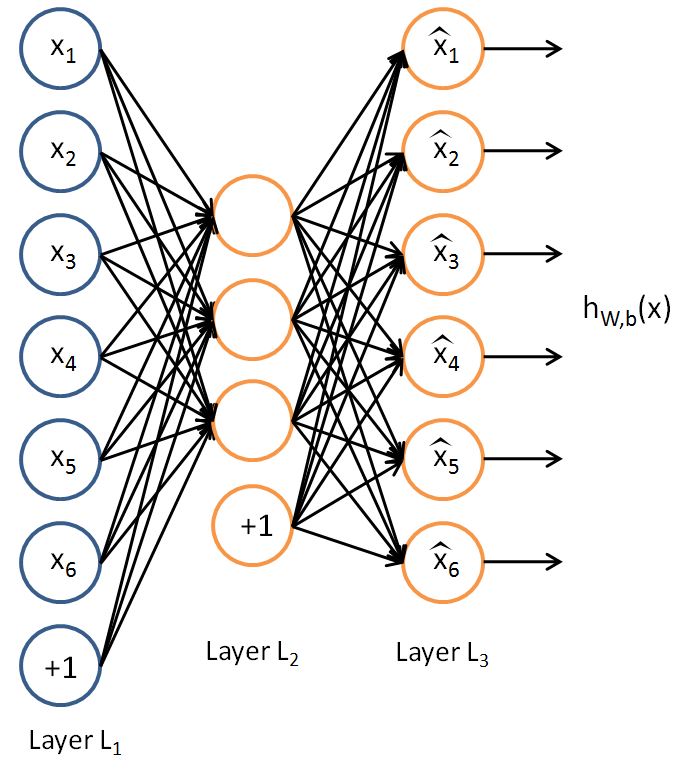
\includegraphics[scale=0.2]{Autoencoder636.png}}
The autoencoder tries to learn a function $h_{W,b}(x) \approx x $  In other words, 
it is trying to learn an approximation to the identity function, so as to output
$\hat{x}$ that is similar to $x$. The identity function seems a particularly trivial function to be trying to learn; but by placing constraints on the network, such as by limiting the number of hidden units, we can discover interesting structure about the data. As a concrete example, suppose 
the inputs $x$ are the pixel intensity values from a $10 \times 10$ image $(100)$ pixels so
$n = 100$, and there are $s_2 = 50$ hidden units in layer $L_2$. Note that we also have $y in \mathbb{R}_100$.
Since there are only $50$ hidden units, the network is forced to learn a ”compressed” representation of the input. 
I.e., given only the vector of hidden unit activations $a_{(2)} \in \mathbb{R}_50 )$, 
it must try to ”‘reconstruct”’ the 100-pixel input $x$ If the input were completely random—say, each $x_i$
comes from an IID Gaussian independent of the other features—then this compression task would be very difficult.
But if there is structure in the data, for example, if some of the input features are correlated, then this algorithm will be able to discover some of those correlations. 
In fact, this simple autoencoder often ends up learning a low-dimensional representation very similar to PCAs.
\\
\paragraph{}
Our argument above relied on the number of hidden units $s_2$
being small. But even when the number of hidden units is large (perhaps even greater than the number of input pixels), we can still discover interesting structure, by imposing other constraints on the network. In particular, if we impose a ”‘sparsity”’ constraint on the hidden units, then the autoencoder will still 
discover interesting structure in the data, even if the number of hidden units is large.\\

\paragraph{}
Informally, we will think of a neuron as being “active” 
(or as “firing”) if its output value is close to 1, 
or as being “inactive” if its output value is close to 0. 
We would like to constrain the neurons to be inactive most of the time. This discussion assumes a sigmoid activation function. If you are using a tanh activation function, then we think of a neuron as being inactive when it outputs values close to -1.\\


\paragraph{}
Recall that $(a_j^2)$ denotes the activation of hidden unit ${j}$
in the autoencoder. However, this notation doesn’t 
make explicit what was the input $x$ that led to that activation. Thus, we will write
$(a_j^2)(x)$ to denote the activation of this hidden unit when the network is given a specific input $(x)$
Further, let\\
\begin{equation}
    \hat{p}_j = \frac{1}{m}\sum_{i=1}^m \bigg [ a_j^{(2)}(x^{(j)}) \bigg ]
     \end{equation}
be the average activation of hidden unit $j$ (averaged over the training set). We would like to (approximately) enforce the constraint
\begin{equation}
\hat{p}_j = \rho 
     \end{equation}
\paragraph{}
where $\rho$ is a ”‘sparsity parameter”’, typically a small value close to zero 
(say $\rho = \bm{0.05}$).In other words, we would like the average activation of each hidden neuron $j$
to be close to 0.05 (say). To satisfy this constraint, the hidden unit’s activations must mostly be near 0.
\paragraph{}
To achieve this, we will add an extra penalty term to our optimization objective that penalizes
$\hat{p}_j$deviating significantly from $\rho$ Many choices of the penalty term will give reasonable results. 
We will choose the following:
\begin{equation}
    \sum_{j=1}^{s=2}\rho \log\frac{p}{\hat{p}_j} + (1 - \rho)\log\frac{1 - \rho}{1 - \hat{\rho}_j}    
    \end{equation}

\paragraph{}
Here, $s_2$is the number of neurons in the hidden layer, and the index $j$
is summing over the hidden units in our network. If you are familiar with the concept of KL divergence, 
this penalty term is based on it, and can also be written
\begin{equation}
    \sum_{j=1}^{s=2}KL(\rho || \hat{\rho}_j)
    \end{equation}
where $KL(\rho || \hat{\rho}_j) = \rho \log\frac{p}{\hat{p}_j} + (1 - \rho)\log\frac{1 - \rho}{1 - \hat{\rho}_j}$
is the Kullback-Leibler (KL) divergence between a Bernoulli random variable with mean $\rho$
and a Bernoulli random variable with mean $\hat{\rho}_j$. KL-divergence is a standard function for measuring how different two different distributions are. (If you’ve not seen KL-divergence before, don’t worry about it; everything 
you need to know about it is contained in these notes.)
\paragraph{}
This penalty function has the property that $KL(\rho || \hat{\rho}_j) = 0$ if $\hat{\rho}_j = \rho$, and otherwise it 
increases monotonically as $\hat{\rho}_j$ diverges from $\rho$. For example, in the figure below, we have set $\rho = \bm{0.02}$ 
and plotted $KL(\rho || \hat{\rho}_j)$ for a range of values of $\hat{\rho}_j:$
\centerline{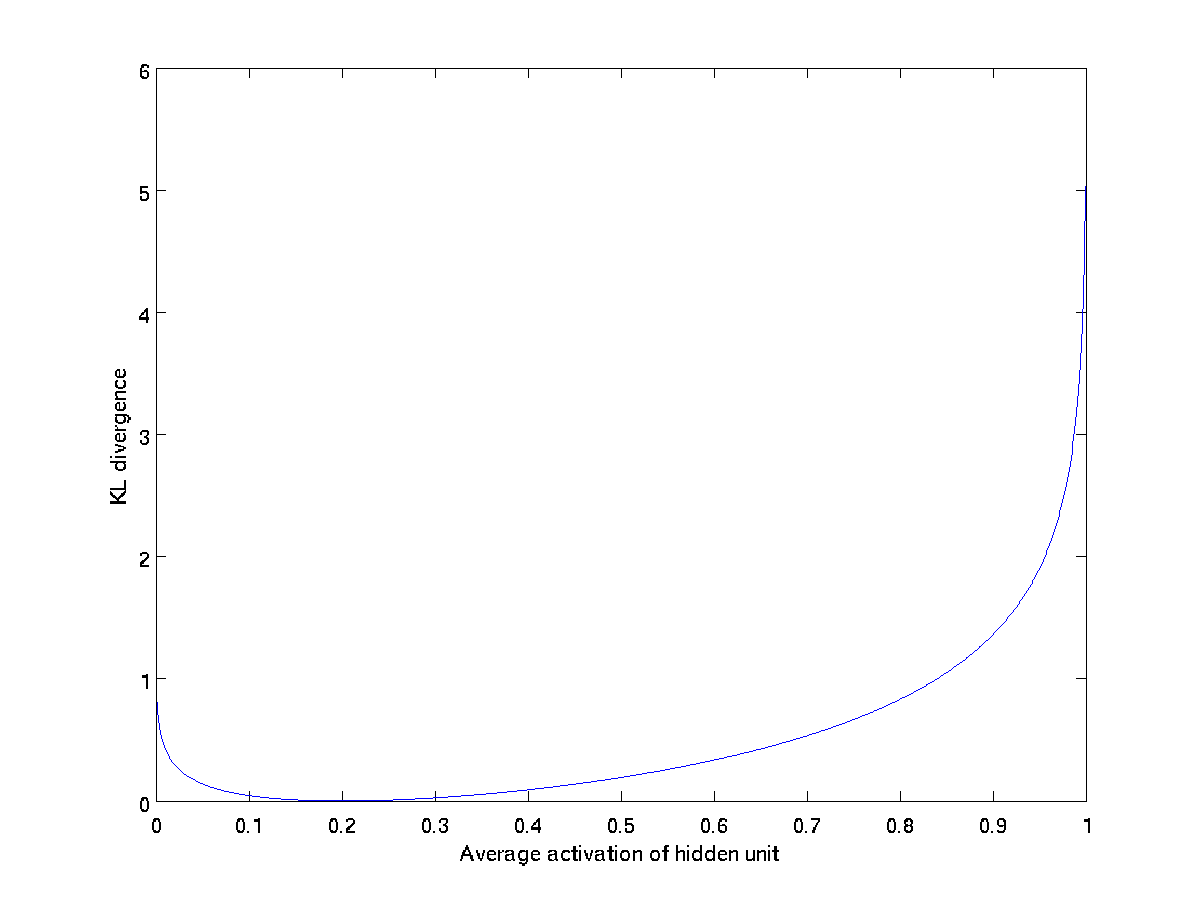
\includegraphics[scale=0.4]{KLPenaltyExample.png}}
We see that the KL-divergence reaches its minimum of 0 at
\begin{equation}
    \hat{\rho}_j = \rho
    \end{equation}
, and blows up (it actually approaches $\infty$ as $\hat{\rho}_j$ approaches 0 or 1. Thus, minimizing this 
penalty term has the effect of causing $\hat{\rho}_j$  to be close to $\rho$.\\
Our overall cost function is now 
\begin{equation}
    J_{sparse}(W,b) = J(W,b) + \beta KL(\rho || \hat{\rho}_j)
    \end{equation}
where $J(W,b)$  is as defined previously, and $\beta$  controls the weight of the sparsity penalty term. The term
$\hat{\rho}_j$ (implicitly) depends on $W,b$  also, because it is the average activation of hidden unit $j$
and the activation of a hidden unit depends on the parameters $W,b$.\\
To incorporate the KL-divergence term into your derivative calculation, there is a simple-to-implement trick involving only a small change to your code. 
Specifically, where previously for the second layer $(l = 2)$, during backpropagation you would have computed
\begin{equation}
    \delta_i^{(2)} = \biggl(\sum_{j=1}^{s2} W_{ji}^{(2)} \delta_j^{(3)} f'(z_i^{(2)}) \biggr)
    \end{equation}
now instead compute
\begin{equation}
    \delta_i^{(2)} = \biggl( \biggl(\sum_{j=1}^{s2} W_{ji}^{(2)} \delta_j^{(3)}\biggr) + \beta \biggl( -\frac{\rho}{\hat{\rho}_i} +  \frac{1-\rho}{1 - \hat{\rho}_i}\biggr) \biggr)f'(z_i^{(2)})
    \end{equation}

One subtlety is that you’ll need to know $\hat{\rho}_i$ to compute this term. 
Thus, you’ll need to compute a 
forward pass on all the training examples first to 
compute the average activations on the training set, 
before computing backpropagation on any example. 
If your training set is small enough to fit comfortably in computer memory 
(this will be the case for the programming assignment), 
you can compute forward passes on all your examples 
and keep the resulting activations in memory and compute the $\hat{\rho}_i$s.
Then you can use your precomputed activations to perform backpropagation on all your examples. If your data is too large to fit in memory, you may have to scan through your examples computing a 
forward pass on each to accumulate (sum up) the activations and compute $\hat{\rho}_i$ (discarding the result 
of each forward pass after you have taken its activations $\hat{a}_i^{(2)}$ into account for computing $\hat{\rho}_i$
). Then after having computed $\hat{\rho}_i$ , you’d have to redo the forward pass for each example so that you can do backpropagation on that example. In this latter case, you would end up computing a 
forward pass twice on each example in your training set, 
making it computationally less efficient.\\
The full derivation showing that the algorithm above results 
in gradient descent is beyond the scope of these notes.
But if you implement the autoencoder 
using backpropagation modified this way, 
you will be performing gradient descent exactly on the
objective $J_sparse(W,b)$. Using the derivative checking method, you will be able to verify this for yourself as well.

\section{Visualizing a Trained Autoencoder}
\paragraph{}
Having trained a (sparse) autoencoder, 
we would now like to visualize the function learned 
by the algorithm, 
to try to understand what it has learned. 
Consider the case of training an autoencoder on
$10 \dot 10$images, so that $n = 10$. Each hidden unit i computes a function of the input:
\begin{equation}
    \hat{a}_i^{(2)} = f \Biggl( \sum_{j=1}^{100} W^{(1)}x_j + b_i^{(1)} \Biggr)
    \end{equation}
We will visualize the function computed by hidden unit $i$—which depends on the parameters
$W_{ij}^{(1)}$(ignoring the bias term for now)—using a 2D image. In particular, we think of 
$\hat{a}_i^{(2)}$ as some non-linear feature of the input $x$. We ask: What input image $x$ would cause 
$\hat{a}_i^{(2)}$ to be maximally activated? (Less formally, what is the feature that hidden unit $i$
is looking for?) For this question to have a non-trivial answer, we must impose some constraints on $x$. If we suppose that the input is norm constrained by 
$\lvert x_{2} \rvert \sum_{i=1}^{100} x_i^{2} \leq 1 $ , then one can show (try doing this yourself) that the input which maximally activates hidden unit 
i is given by setting pixel $x_j$  (for all 100 pixels, $j=1,\dots100$) to
\begin{equation}
    x_j = \frac{W_{ij}^{(1)}}{\sqrt{\sum_{j=1}^{(100)}W_{ij}^{(2)}}}
    \end{equation}
By displaying the image formed by these pixel intensity values, we can begin to understand what feature hidden unit
$i$is looking for.\\ \\
If we have an autoencoder with 100 hidden units (say), then we our visualization will have 100 such images—one per hidden unit. By examining these 100 images, we can try to understand what the ensemble of hidden units is learning.\\
When we do this for a sparse autoencoder (trained with 100 hidden units on 10x10 pixel inputs1 we get the following result:\\ \\
\centerline{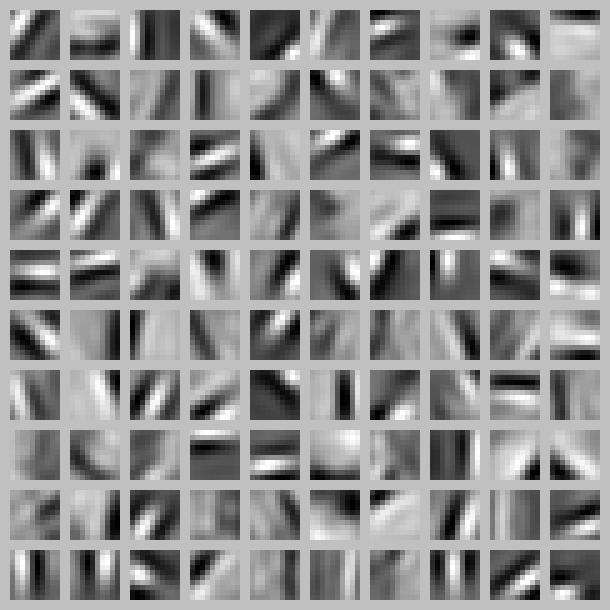
\includegraphics[scale=0.38]{ExampleSparseAutoencoderWeights.png}}
Each square in the figure above shows the (norm bounded) input image x that maximally actives one of 100 hidden units. We see that the different hidden units have learned to detect edges at different positions and orientations in the image.\\ \\
These features are, not surprisingly, useful for such tasks as object recognition and other vision tasks. When applied to other input domains (such as audio), this algorithm also learns useful representations/features for those domains too.\\ \\
1”The learned features were obtained by training on ”‘whitened”’ natural images. Whitening is a preprocessing step which removes redundancy in the input, by causing adjacent pixels to become less correlated.
\end{document}
